\documentclass[a4]{jarticle}
%\usepackage{html,htmllist}
\usepackage{lgrind}
%\usepackage[dvips]{graphicx,color}
\usepackage[dvipdfmx]{graphicx,color}
\usepackage{amsmath}
\usepackage{amsthm}

\topmargin=-2.0cm
\textheight=25.0cm
\textwidth=17.0cm
\oddsidemargin=-1.0cm
\evensidemargin=-1.0cm
\renewcommand{\baselinestretch}{0.95}%ページ数が伸びたときにはここに
%1.0以下の数字を入れてみましょう

\title{Operating Instruction of Zheng Yufei}
%\author{B4 鄭 中翔} %名前、学年を入れましょう
\author{鄭 雨霏} %名前、学年を入れましょう

\begin{document}
    \twocolumn{
    \maketitle
    }

    \section{Factory Settings}

    %\begin{enumerate}
    %\item 研究背景(はじめに)
    %\item 研究目的
    %\item 関連研究紹介か実験計画か実験結果
    %\item 参考文献
    %\end{enumerate}

    Zheng Yufei, born in April 18th, 1996, female. Her name in Chinese means "raining so big".
    You can call her "Fei chyan". She graduated from
    Sun Yat-sen University in 2014. Her undergraduate major is Mathematics
    and Applied Mathematics. She has very broad interests but none of
    them is professional. Although she is a quick learner and good at
    asking questions, she likes to procrastinate her work. If anyone
    finds her absent-minded, please remind her of the work must to be
    done and tell her the dead line is very close. Her built-in programs
    don't include human-face-recognition or map navigation. As a result,
    she often gets lost and suffer from face blindness.

    \section{Features and Preferences}

    Zheng Yufei has many showy and not substantial skills, including singing,
    playing the piano, playing the violin, drawing, playing various courtgames
    and so on. After many years of coding, most of them have been forgotten
    successfully. If you're interested, you can talk to her to find more
    information. For the moment, she likes playing video games and watching
    Japanese animations. She will be so happy if you let her know that you
    are playing a same game. Zheng yufei doesn't like drinking because she
    is allergic to alcohol, and very picky about what to eat. She has two cats in
    her family. She is very happy to show other people the pictures of her cats.
    Try to ask her for more information about it. You can choose to speak
    Japanese or English to her, of course Chinese is the best. Both of her spoken
    English and Japanese are not very well, but she is trying to communicate
    better with others, please help her if you want.

    \begin{figure}
        \begin{center}
            \centering
            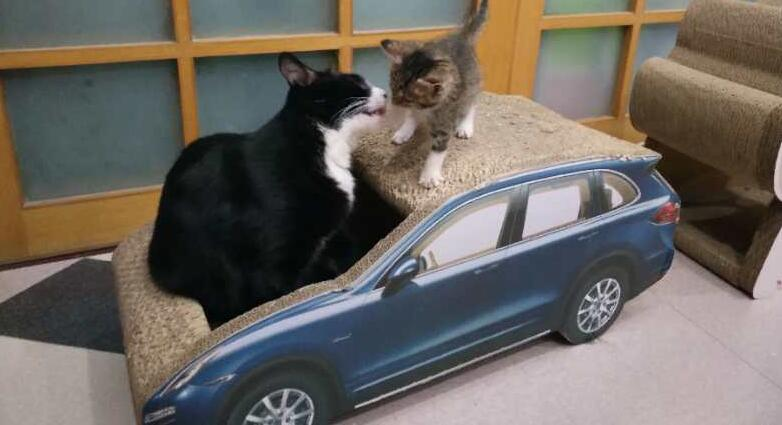
\includegraphics[width=\linewidth]{cats.jpg}
            \caption{Zheng Yufei's cats}
            \label{fig:mcmthesis-logo}
        \end{center}
    \end{figure}

    \section{Application Status}
    Zheng Yufei has been tried many programming
    languages, but be careful, she
    couldn't make out the difference between the languages but only know how
    to compile them without making errors. She tried her best to completed many basic computer courses. So she is able
    to understand the basic technical communication. She doesn't have some brilliant
    deeds, mostly just to amuse herself by writing some little video games.
    If you're interested and don't mind the quality of the games, you can ask her
    for a copy.(Only for Windows and Android). She's completely new to CG, ML and
    Java, so she may ask a lot of questions about these things, please don't get
    bored. She always fancy that she could combine her awful drawings with the
    models, while currently she doesn't know how to do. Her current and
    biggest experiment is her undergraduate graduation project with many, many bugs.
    If you are curious, you can go to ask her and try it out. It would be nice
    if you could give her some help.

    \section{Conclusion}

    It looks like a little bit of trouble, all in all, Zheng Yufei is
    very easy to get along with, don't worry. There's always something
    wrong with being a new guys, so please to understand more. If you
    have more questions, please feel free to contact with her.
    Hope you'll have a good cooperation together.


\end{document}
